\documentclass[a4paper, 12pt]{article}
\usepackage{fontspec}
%\usepackage[utf8]{inputenc}
\usepackage{graphicx}
\usepackage{float}
\usepackage{hyperref}
\usepackage[margin=2cm]{geometry}
\usepackage{amsmath}
\usepackage[polish]{babel}
\usepackage[nottoc,numbib]{tocbibind}
%\usepackage{polski}


\title{\textbf{Symulacja ruchu ludzi w centrum handlowym}}
\author{Paweł Kłeczek \\ \emph{pkleczek@student.agh.edu.pl} \and Kajetan Rzepecki \\ \emph{kajetan.rzepecki+agh@gmail.com}}
\date{\today}

\begin{document}

    \maketitle

    \vfill
    \begin{abstract}
    % TODO Trzeba dodać coś więcej IMO, na przykład o tym, jak podejdziemy do problemu ruchu ludzi.

\noindent
Praca i związany z nią projekt dotyczą symulowania ruchu ludzi w centrum handlowym z wykorzystaniem modelu \emph{Social Distances} na dwuwymiarowej siatce.
    \end{abstract}
    \vfill

    \thispagestyle{empty} % Nie chcemy numerować pierwszej strony.

\newpage
    \setcounter{page}{1}
    \setcounter{tocdepth}{3}

    \tableofcontents

\newpage
    \section{Wprowadzenie}
    \label{sec:intro}

\noindent
Celem wykonywanego projektu jest stworzenie modelu oraz symulacja ruchu ludzi w centrum handlowym w oparciu między innymi o model \emph{Social Distances} (\cite{refs:social-distances-1, refs:social-distances-2}).

Modelowanie ruchu dużych grup ludzi w środowisku centrum handlowego jest problemem złożonym i wymaga wykorzystania równie złożonych algorytmów celem dokładnego przybliżenia rzeczywistych zachowań. Dobrym podejściem jest dekompozycja problemu modelowania złożonego zjawiska na mniejsze, łatwiejsze do rozwiązania podproblemy, którymi zajmują się osobne, dobrze zdefiniowane i wyspecjalizowane algorytmy, i ponowne połączenie wyników ich działania w spójną całość - metoda \emph{Divide and Conquer}.

    \begin{figure}[H]
        \centering
        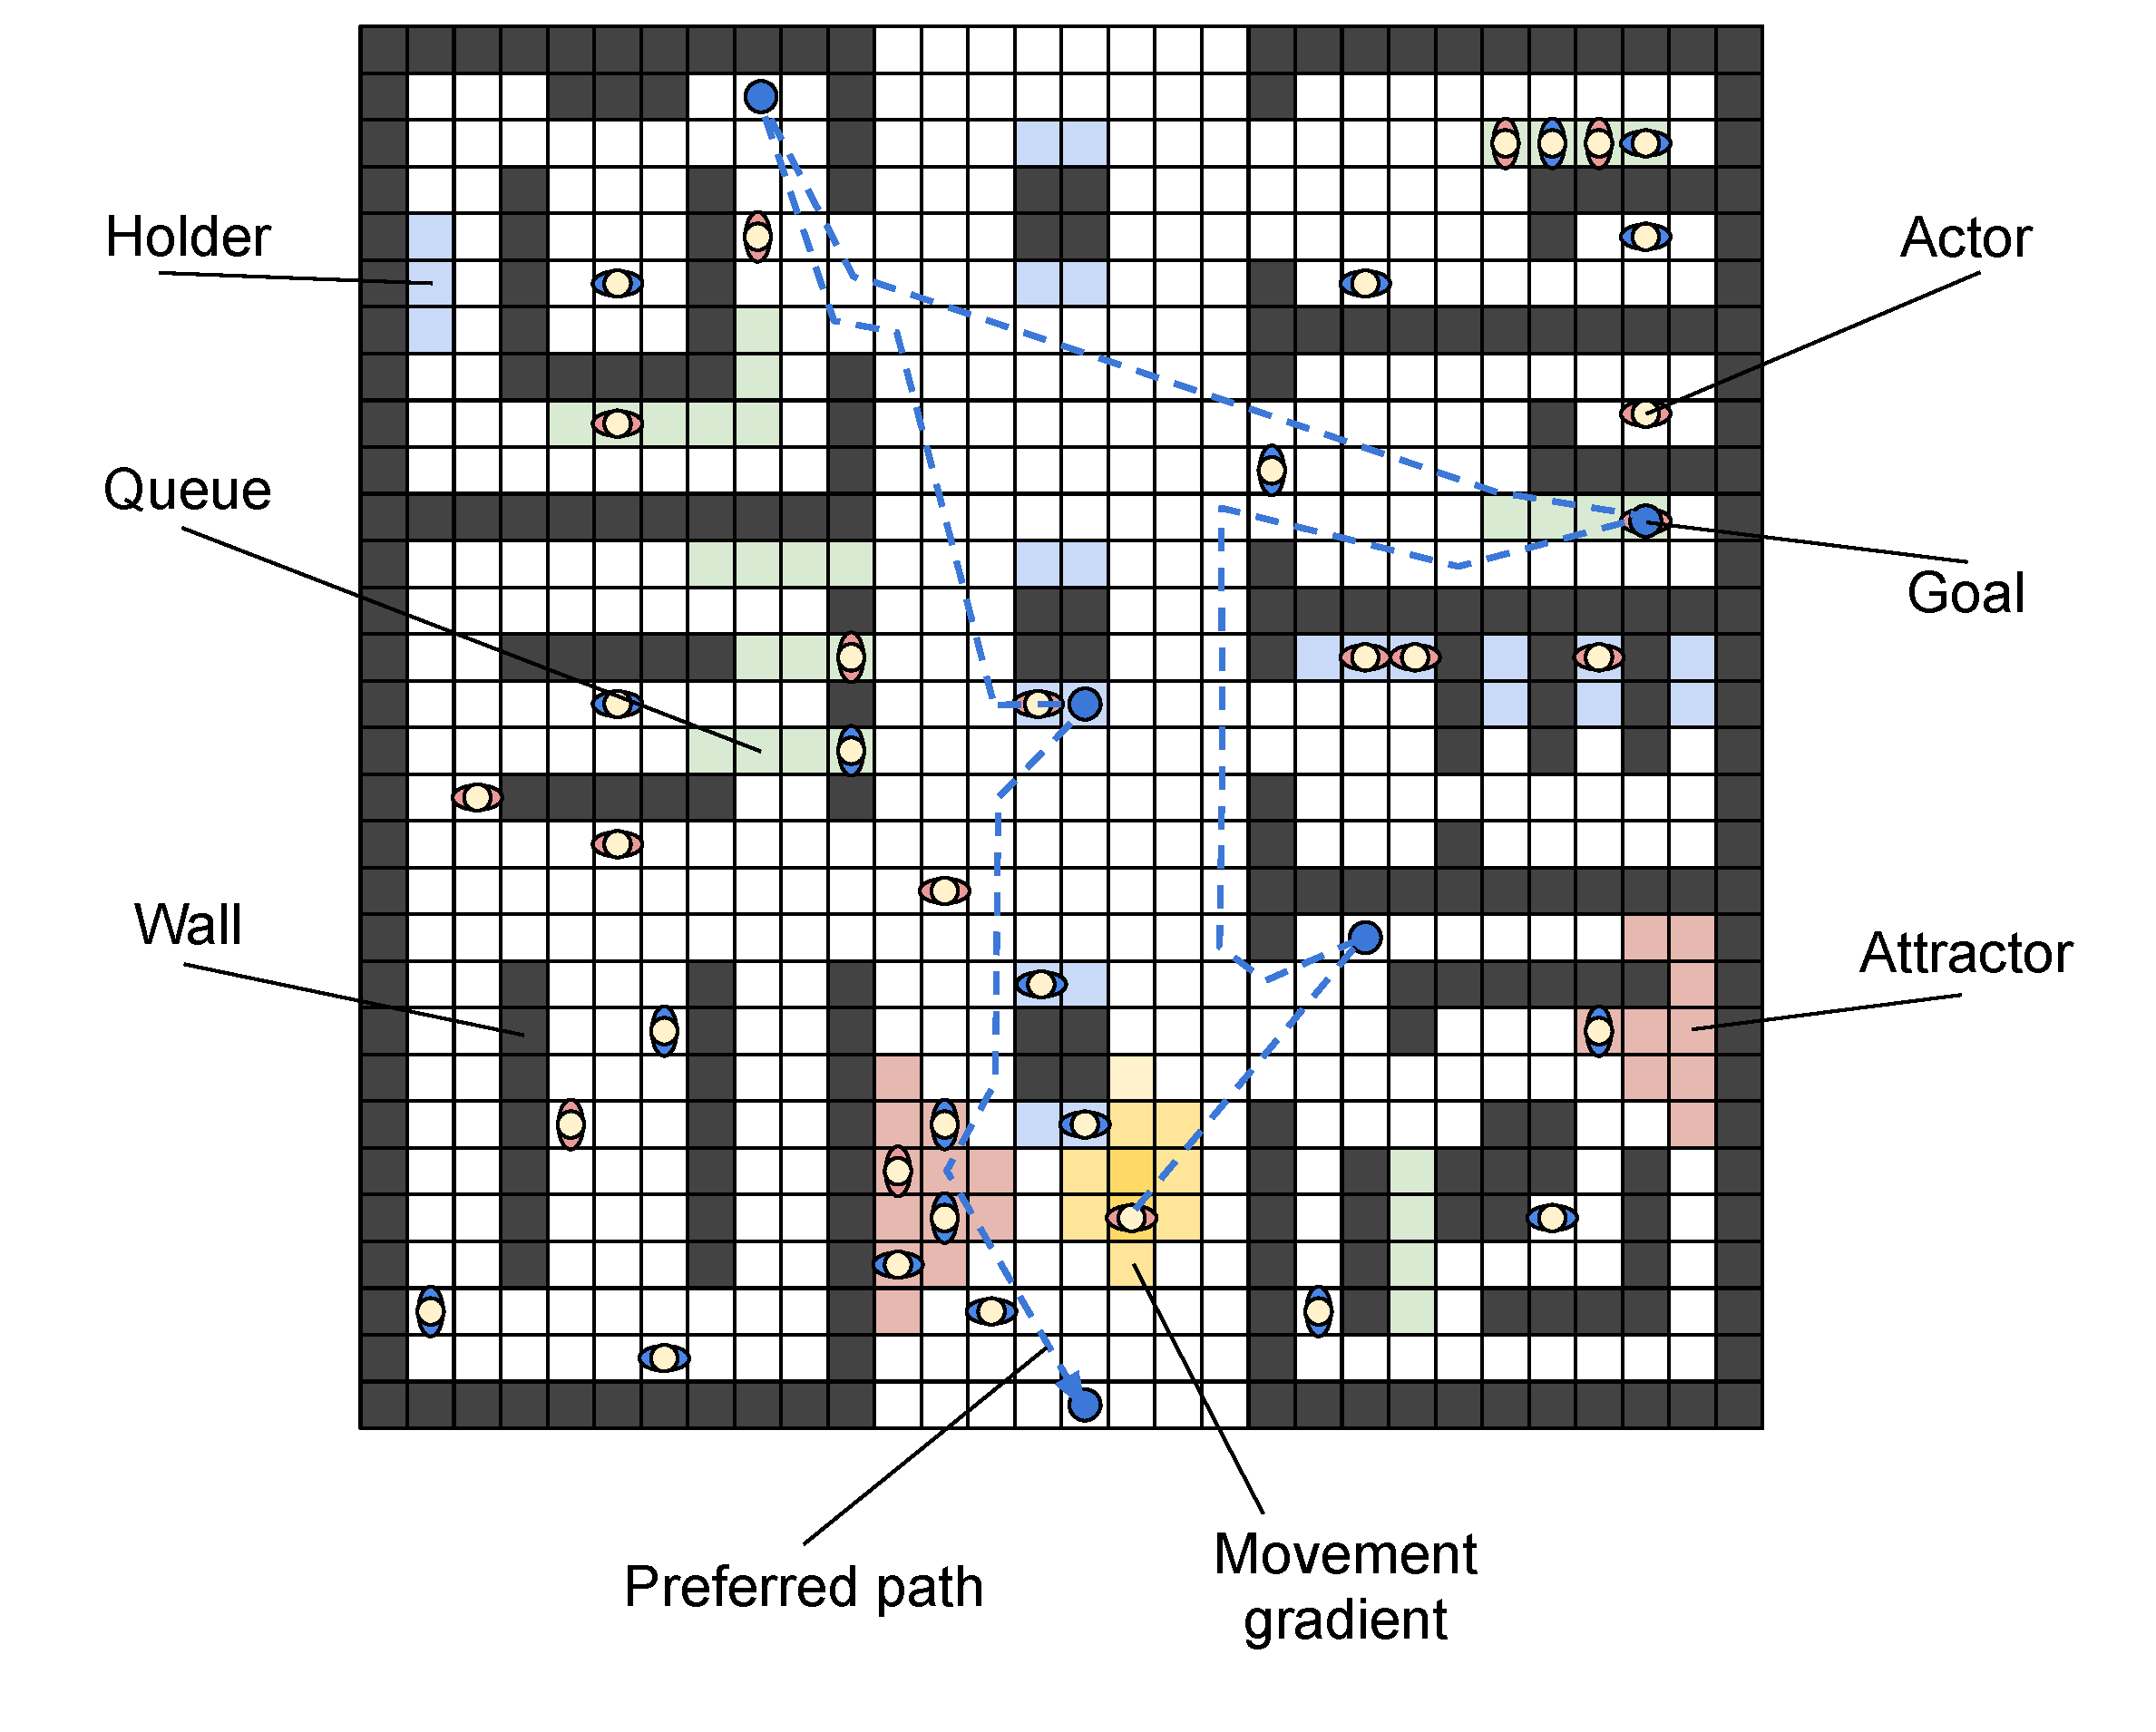
\includegraphics[scale=0.3]{./img/Overview.pdf}
        \caption{Przykładowa dekompozycja problemu modelowania ruchu ludzi w centrum handlowym.}
        \label{fig:decomp}
    \end{figure}

W zależności od domeny rozwiązywanego problemu dekompozycja może zachodzić ze względu na wiele czynników i dotyczyć różnych aspektów problemu - np. podział wejściowego zbioru danych na dwa mniejsze podzbiory w algorytmie \emph{Quick sort}, czy podział modelu ruchu ludzi na elementarne zachowania, jak \emph{kolejkowanie}, \emph{atrakcja} lub \emph{oczekiwanie}.

Na rysunku \ref{fig:decomp} została przedstawiona przykładowa dekompozycja problemu poruszanego w tym dokumencie. Wyszczególniono w niej podział na globalną, preferowaną ścieżkę wiodącą poruszającego się po centrum handlowym agenta do obranych przez niego celów i lokalny ruch zgodny z gradientem ruchu obliczonym na podstawie jego otoczenia. Dodatkowo zastosowano podział na specjalne strefy odpowiedzialne za modelowanie elementarnych zachowań ludzi w centrach handlowych, takie jak strefy kolejek, czekania i gromadzenia się, które realizowane są za pomocą innych modeli ruchu.

\newpage
    \subsection{State of the art}
    \label{sec:sota}

\noindent
Zagadnienia modelowania ruchu ludzi są od długiego czasu postrzegane jako istotne z punktu widzenia usługowego. Już w latach 80 ubiegłego wieku Aloys Borgers i Harry Timmermans zajmowali się modelowaniem ruchu pieszych w środowisku centrum handlowego w oparciu o modele probabilistyczne (\cite{refs:route-choice-1}).
Na przestrzeni lat modele ruchu pieszych ewoluowały w wielu kierunkach, od dynamiki płnów (\cite{refs:fluid-dynamics}) przez automaty komórkowe (\cite{refs:cellular-movement}) i algorytmy genetyczne (\cite{refs:pedestrian-behaviour-2}) aż do modeli opartych o systemy wieloagentowe (\cite{refs:real-data-2}). \\

\emph{Cellular automata microsimulation for modeling bi-directional pedestrian walkways} \linebreak (\cite{refs:cellular-movement}) skupia się na modelowaniu dwukierunkowego ruchu ludzi z wykorzystaniem automatów komórkowych. Praca ta dowodzi, że stosunkowo nieskomplikowany automat komórkowy z małą liczbą reguł jest zdolny do symulowania skomplikowanych zachowań, które dobrze oddają rzeczywistość. Zaproponowany model i algorytm \textbf{CA-ped} pozwalają symulować ruch ludzi w dwóch przeciwnych kierunkach na dwóch oddzielnych jak i mieszanych pasach ruchu, a także dynamicznych, wieloliniowych (\emph{dynamic multi-lane, DML}) pasach ruchu.

Algorytm \textbf{CA-ped} wyróżnia dwie fazy ruchu, z których każda charakteryzuje się trzema prostymi zasadami:

\begin{enumerate}
    \item Zmiana pasa ruchu
        \begin{itemize}
            \item Eliminacja konfliktów - dwóch przechodniów nie może znajdować się na jednej komórce, w przypadku konfliktu wolna komórka oddzielająca dwóch przechodniów jest przyznawana jednemu z nich z równym prawdopodobieństwiem.
            \item Identyfikacja wolnych przestrzeni - wybierany jest ten pas ruchu, który cechuje największa liczba wolnych komórek, co implikuje bezproblemowy ruch w przyszłości.
            \item Zmiana pasa - każdy przechodzień jest poruszany na jeden z dwóch sąsiednich pasów, lub pozostaje na obecnym pasie ruchu.
        \end{itemize}
    \item Ruch do przodu
        \begin{itemize}
          \item Obliczanie szybkości ruchu - dla każdego przechodnia obliczana jest jego szybkość uzależniona od istnienia, bądź nie, wolnych komórek w jego otoczeniu.
          \item Wymijanie - jeśli bezpośrednio przed przechodniem w niedużej odległości istnieje przeciwstawny przechodzień, to z zadanym prawdopodobieństwiem następuje wyminięcie obu przechodniów.
          \item Ruch - każdy przechodzień jest przemieszczany do przodu zgodnie z szybkością jego ruchu.
        \end{itemize}
\end{enumerate}

\emph{Pedestrian behaviour modelling - An application to Retail Movements using a Genetic Algorithm} (\cite{refs:pedestrian-behaviour-2}) identifikuje problemy i nieścisłości wynikające ze stosowania modeli opartych o najkrótsze ścieżki (\emph{shortest-paths}) i maksymalizację przydatności (\emph{utility-maximization}) do symulowania ruchu ludzi w centrum handlowym. Specjalnie zaprojektowany algorytm genetyczny wykorzystuje informacje o optymalnych ścieżkach i mapę routingu i atrybutów konkretnych miejsc centrum handlowego do znalezienia mniej optymalnych ścieżek prowadzących agentów do wybranych przez nich sklepów, które lepiej modelują zachowanie ludzi w środowisku centrum handlowego.

Na podstawie społecznych i ekonomicznych atrybutów poszczególnych miejsc centrum handlowego i atrybutów ludzi przebywających w centrum handlowym, takich jak szybkość, wiek, płeć i przychód, oraz korzystając z mapy routing algorytm wyznacza listę miejsc zainteresowania, które kupujący planują odwiedzić. Następnie z użyciem algorytmu genetycznego wyznaczane są ścieżki obejmujące wszystkie miejsca zainteresowania konkretnego kupującego, które zostają wykorzystane w dalszej części symulacji.
Istotnym jest wyszczególnienie fazy ruchu lokalnego, gdzie zachodzą dodatkowe zjawiska, których nie obejmuje zasięg zastosowanego algorytmu genetycznego. Wspomniane zjawiska to \emph{omijanie przeszkód} (\emph{collision avoidance}) występujących w lokalnym otoczeniu poruszającego się człowika oraz \emph{grupowanie się} (\emph{flocking}), czyli skomplikowane zjawisko przyciągania kupującego do grup innych kupujących zgodnie z jego socjologicznymi preferencjami. \\

\emph{The Simulated Consumer - an Agent-based approach to Shopping Behaviour} \linebreak (\cite{refs:real-data-2}) identyfikuje istnienie dużej liczby różnych schematów zachowań i szeroki zakres problemu modelowania ruchu ludzi w centrum handlowym proponując podejście agentowe jako dostatecznie elastyczną metodę modelowania skomplikowanej dynamiki kupujących. W oparciu o skorelowane w niewielkim stopniu dane pochodzące z północy Szwecji i południa Niemiec autorzy definiują agentowy model wyboru miejsc zainteresowania, który następnie z powodzeniem stosują do symulowania zachowania kupujących w dwóch różnych sektorach - spożywczym i odzieżowym, jednocześnie potwierdzają elastyczność zaproponowanego modelu. \\

Więcej interesujących publikacji związanych z tematyką tego projektu zawarto w secji \ref{sec:refs}.

\newpage
    \section{Model centrum handlowego}
    \label{sec:mall-model}

\noindent
Zgodnie z metodą \emph{Divide and Conquer} zaproponowaną we \hyperref[sec:intro]{wprowadzeniu}, zdecydowano się na dekompozycję problemu modelowania ruchu ludzi w centrum handlowym na elementarne, abstrakcyjne zachowania oraz, ze względu na cele poszczególnych agentów i sposoby ich osiągania, na globalne i lokalne planowanie trasy podróży, co zawarto na rysunku \ref{fig:overview}.

    \begin{figure}[H]
        \centering
        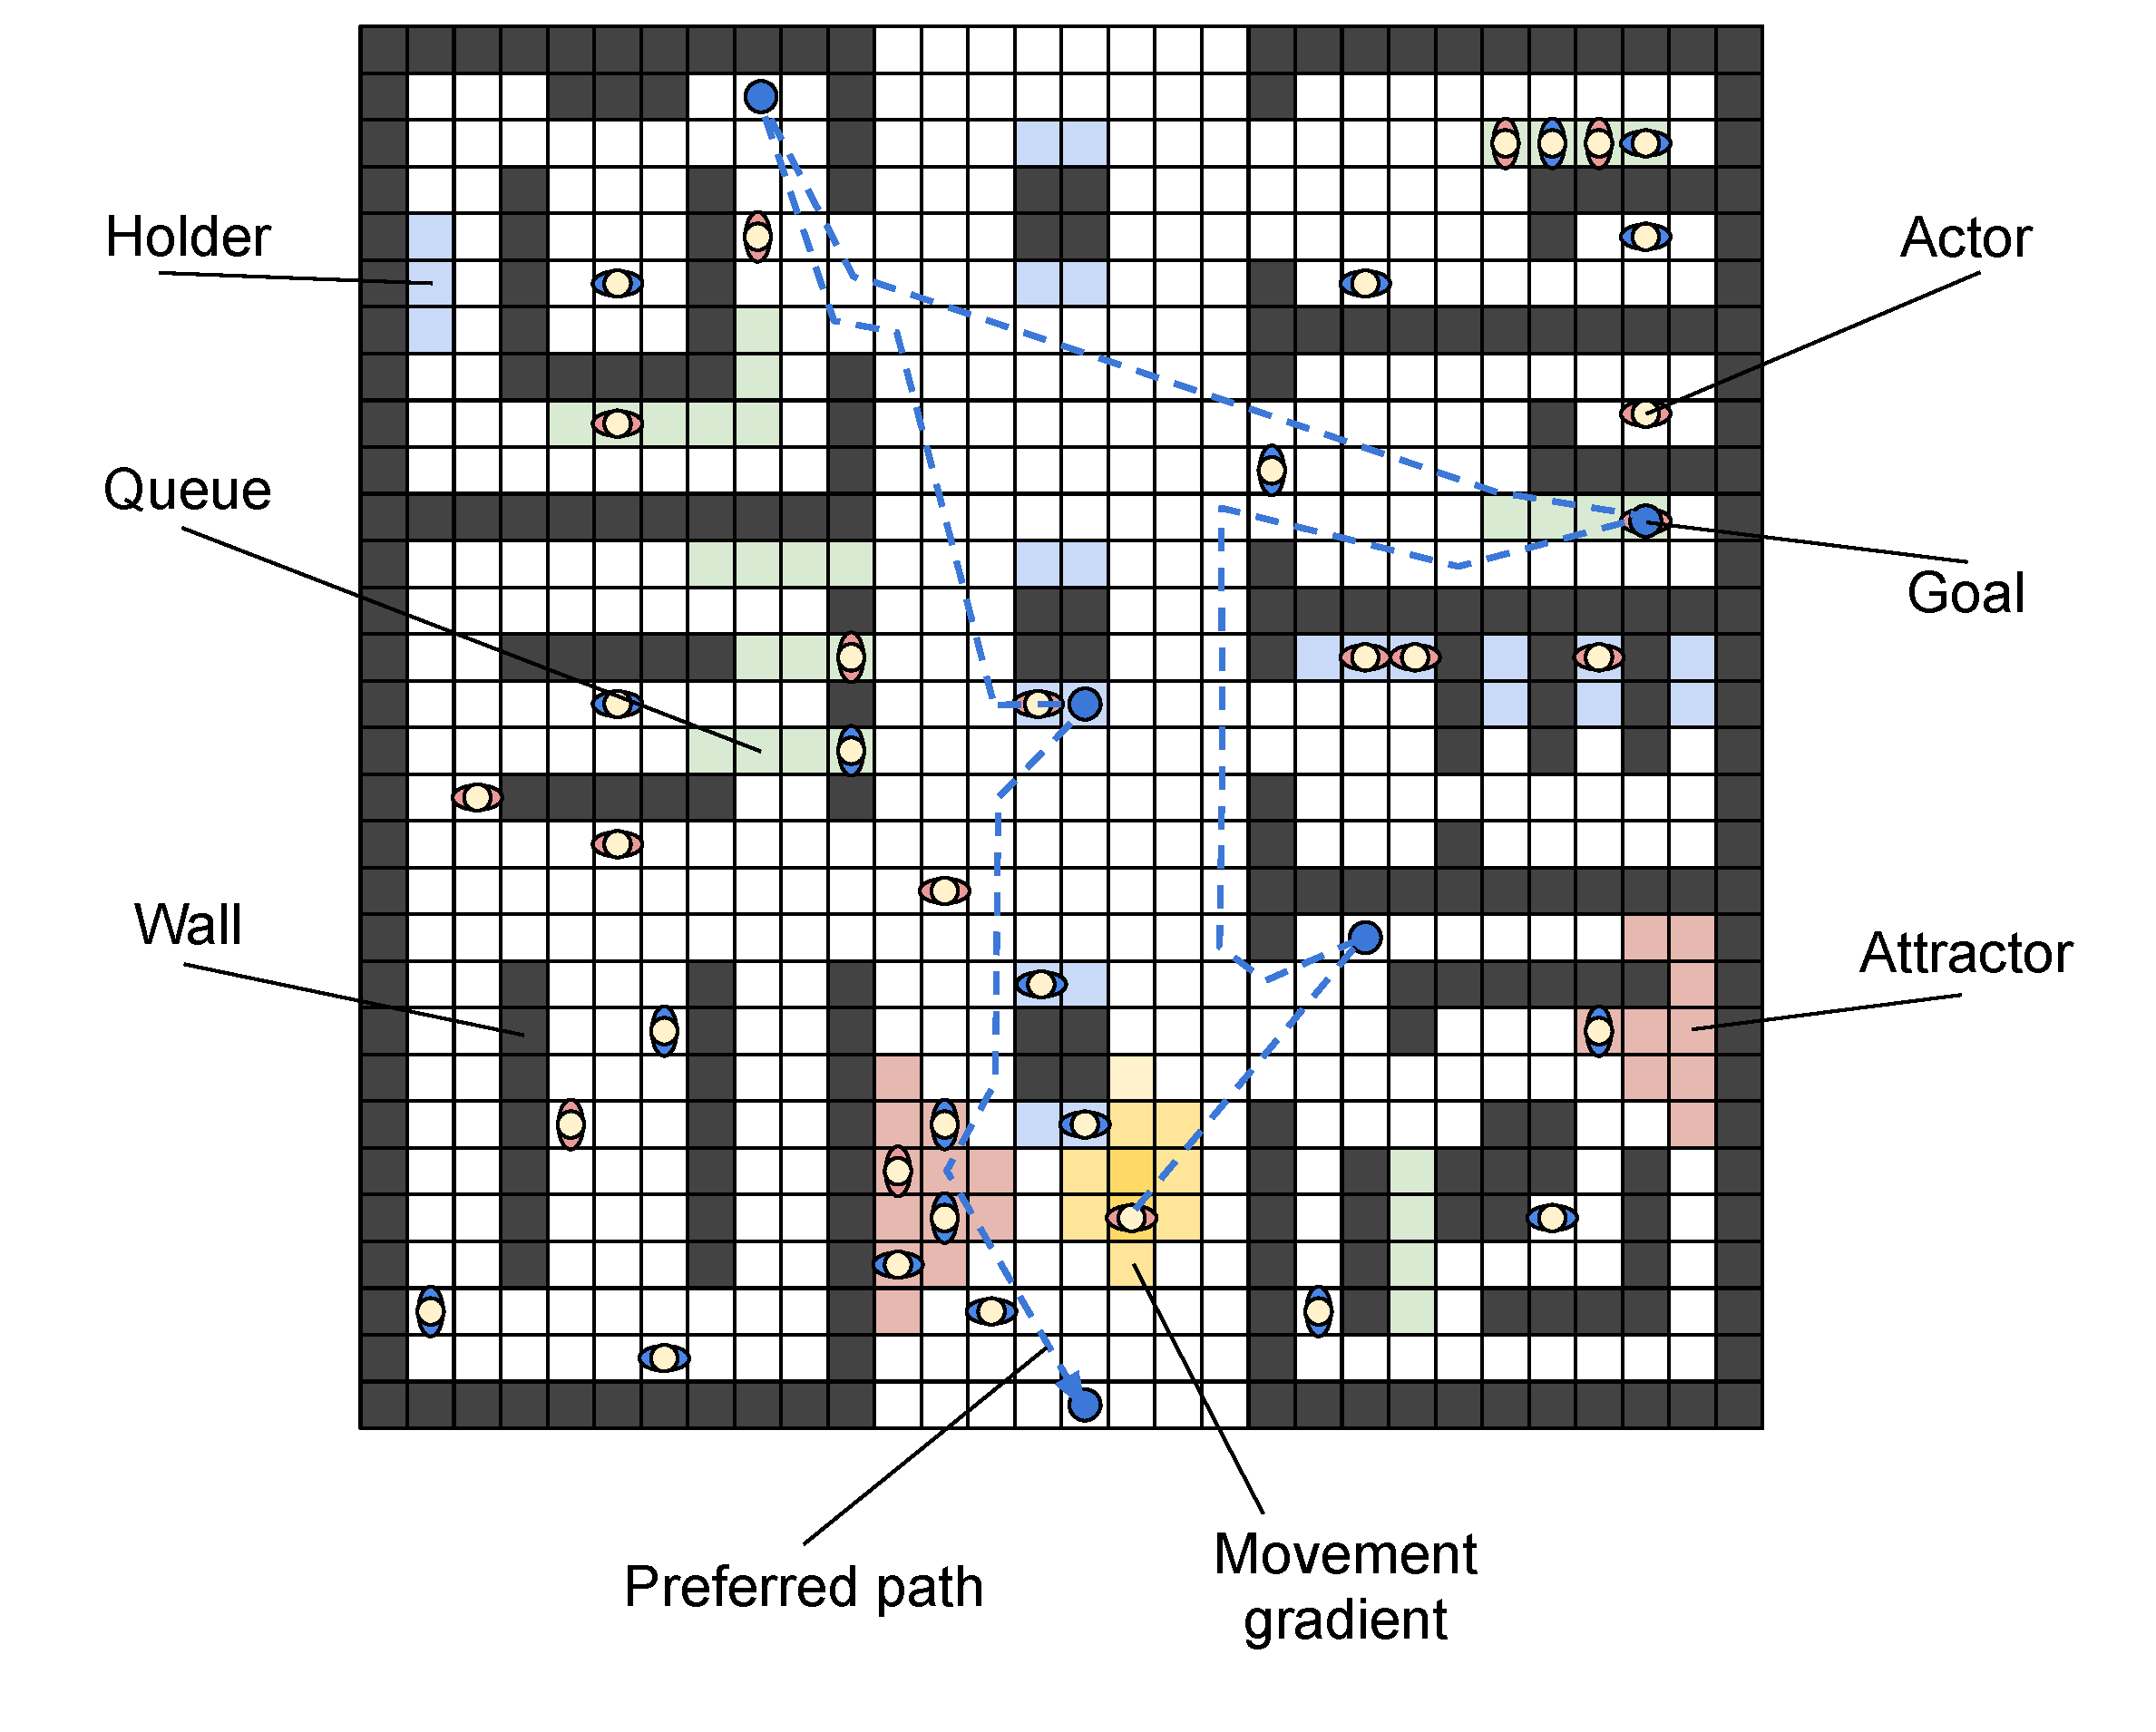
\includegraphics[scale=0.3]{./img/Overview.pdf}
        \caption{Zastosowana dekompozycja problemu.}
        \label{fig:overview}
    \end{figure}

Model centrum handlowego przewiduje istnienie specjalnych stref, wewnątrz których algorytmy odpowiedzialne za poruszanie agentów są modyfikowane lub zastępowane celem modelowania dobrze zdefiniowanych elementarnych zachowań, takich jak \emph{kolejkowanie}, czy \emph{grupowanie się}. W wyniku obserwacji stwierdzono istnienie czterech rodzajów stref specjalnych - strefy przyciągania uwagi (atraktory), kolejki, przejścia i miejsca przeznaczone do czekania.

    \subsection{Atraktory}
    \label{sec:attractors}

Atraktor jest specjalną strefą charakteryzującą się podwyższonym zainteresowaniem ze strony agentów poruszających się po centrum handlowym. Atraktor ma za zadanie modelować obecność przedmiotu lub zjawiska, które przykuwa uwagę ludzi na terenie centrum handlowego, a wynikiem jego działania jest spontaniczne powstawanie skupisk ludzi - \emph{grupowanie się}.

    \begin{figure}[H]
        \centering
        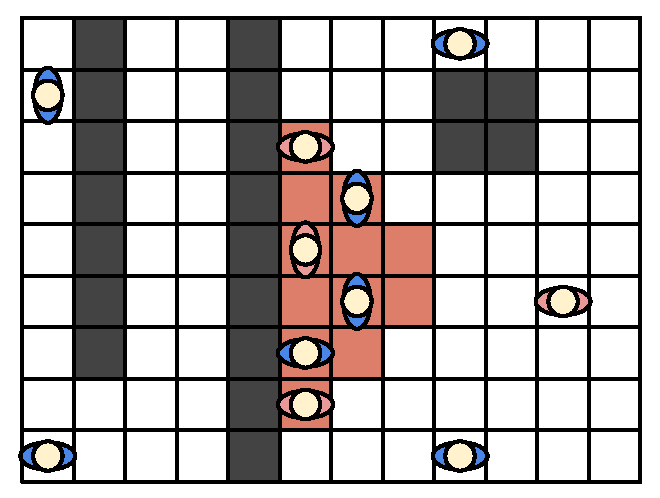
\includegraphics[scale=0.4]{./img/Crowding.pdf}
        \caption{Grupowanie się agentów w obrębie atraktora.}
        \label{fig:crowding}
    \end{figure}

Atraktory różnią się między sobą typami - atraktory różnych typów przyciągają inne rodzaje agentów, co modeluje różnice w preferencjach ludzi przebywających w centrum handlowym. Działanie atraktorów jest najistotniejsze w \hyperref[sec:tactical]{taktycznej} fazie modelu ruchu, w której ma miejsce wybór i modyfikacja preferowanych przez agentów dróg prowadzących do wybranych celów.

    \subsection{Kolejki}
    \label{sec:queues}

Drugim istotnym z punktu widzenia modelu centrum handlowego typem strefy specjalnej jest strefa kolejki. Zadaniem kolejki jest modelowanie zjawiska \emph{ścisłego kolejkowania się} ludzi, na przykład przy kasie sklepowej, lub na stopniach eskalatora, co nie wynika z ogólnego modelu ruchu.

    \begin{figure}[H]
        \centering
        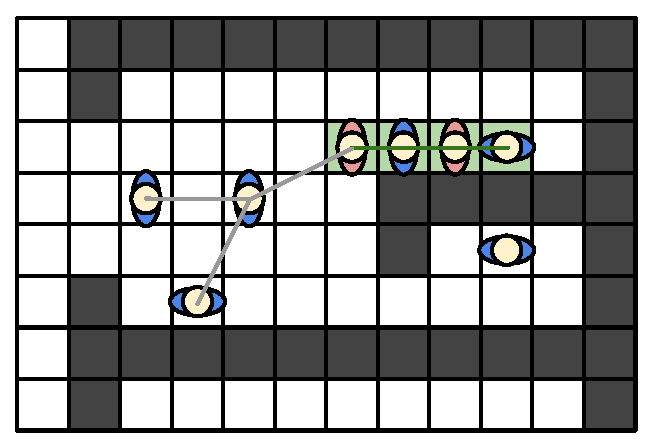
\includegraphics[scale=0.4]{./img/Queueing.pdf}
        \caption{Kolejkowanie się ludzi przy kasie sklepowej z zaznaczoną kolejką ścisłą.}
        \label{fig:queueing}
    \end{figure}

Kolejki modyfikują działanie \hyperref[sec:operational]{fazy operacyjnej} modelu ruchu zmniejszając udział modelu preferencji odległościowych w wyznaczaniu oceny sąsiadujących z agentem komórek mapy centrum handlowego.

    \subsection{Przejścia/wejścia/wyjścia}
    \label{sec:entrance-exits}

Strefy przejść pozwalają na \emph{tworzenie}, \emph{przemieszczanie} pomiędzy różnymi fragmentami mapy centrum handlowego i \emph{usuwanie} agentów, którzy osiągnęli wszystkie cele swojej podróży.

    \begin{figure}[H]
        \centering
        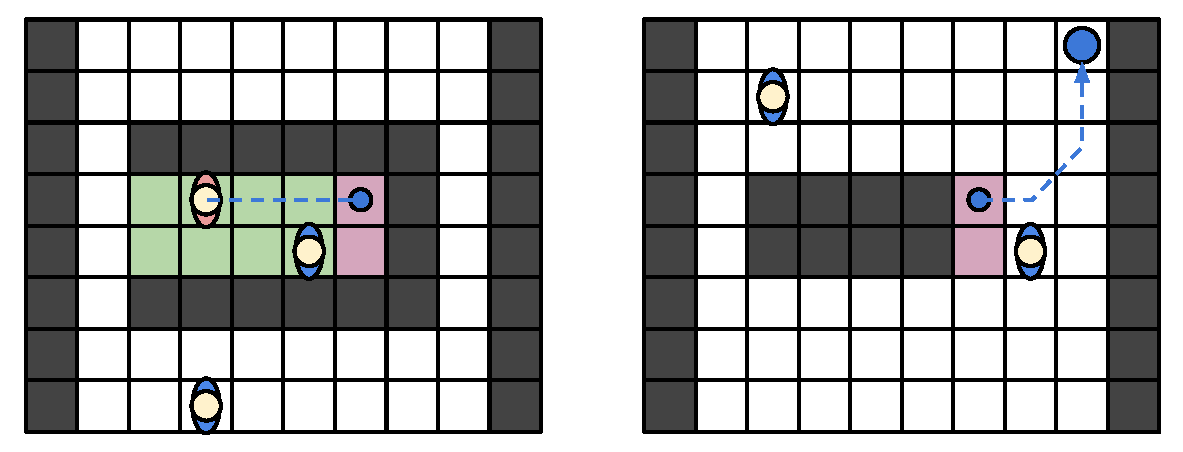
\includegraphics[scale=0.4]{./img/EntranceExits.pdf}
        \caption{Poruszanie się agenta po eskalatorze pomiędzy piętrami centrum handlowego.}
        \label{fig:passing-through}
    \end{figure}

    \subsection{Miejsca oczekiwania}
    \label{sec:holders}

Ostatnim istotnym typem strefy specjalnej jest miejsce oczekiwania, modelujące wszelkiego rodzaju miejsca spędzania czasu w bezruchu. Agent trafiający do miejsca oczekiwania zostaje wstrzymany na ustaloną ilość czasu przed kontynuowaniem swojej podróży.

    \begin{figure}[H]
        \centering
        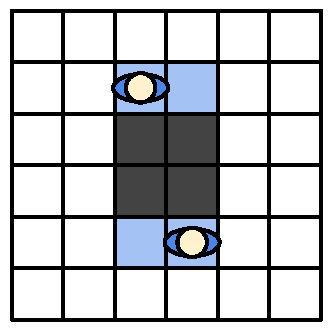
\includegraphics[scale=0.4]{./img/Held.pdf}
        \caption{Agenci oczekujący końca świata.}
        \label{fig:held-down}
    \end{figure}

\newpage
    \section{Model ruchu ludzi}
    \label{sec:move-model}

\noindent
W zastosowanym algorytmie można wyszczególnieć dwie główne, wzajemnie od siebie zależne fazy - fazę \hyperref[sec:tactical]{taktyczną} oraz fazę \hyperref[sec:operational]{operacyjną}, których interakcję przestawiono na poniższym, uproszczonym diagramie.

    \begin{figure}[H]
        \centering
        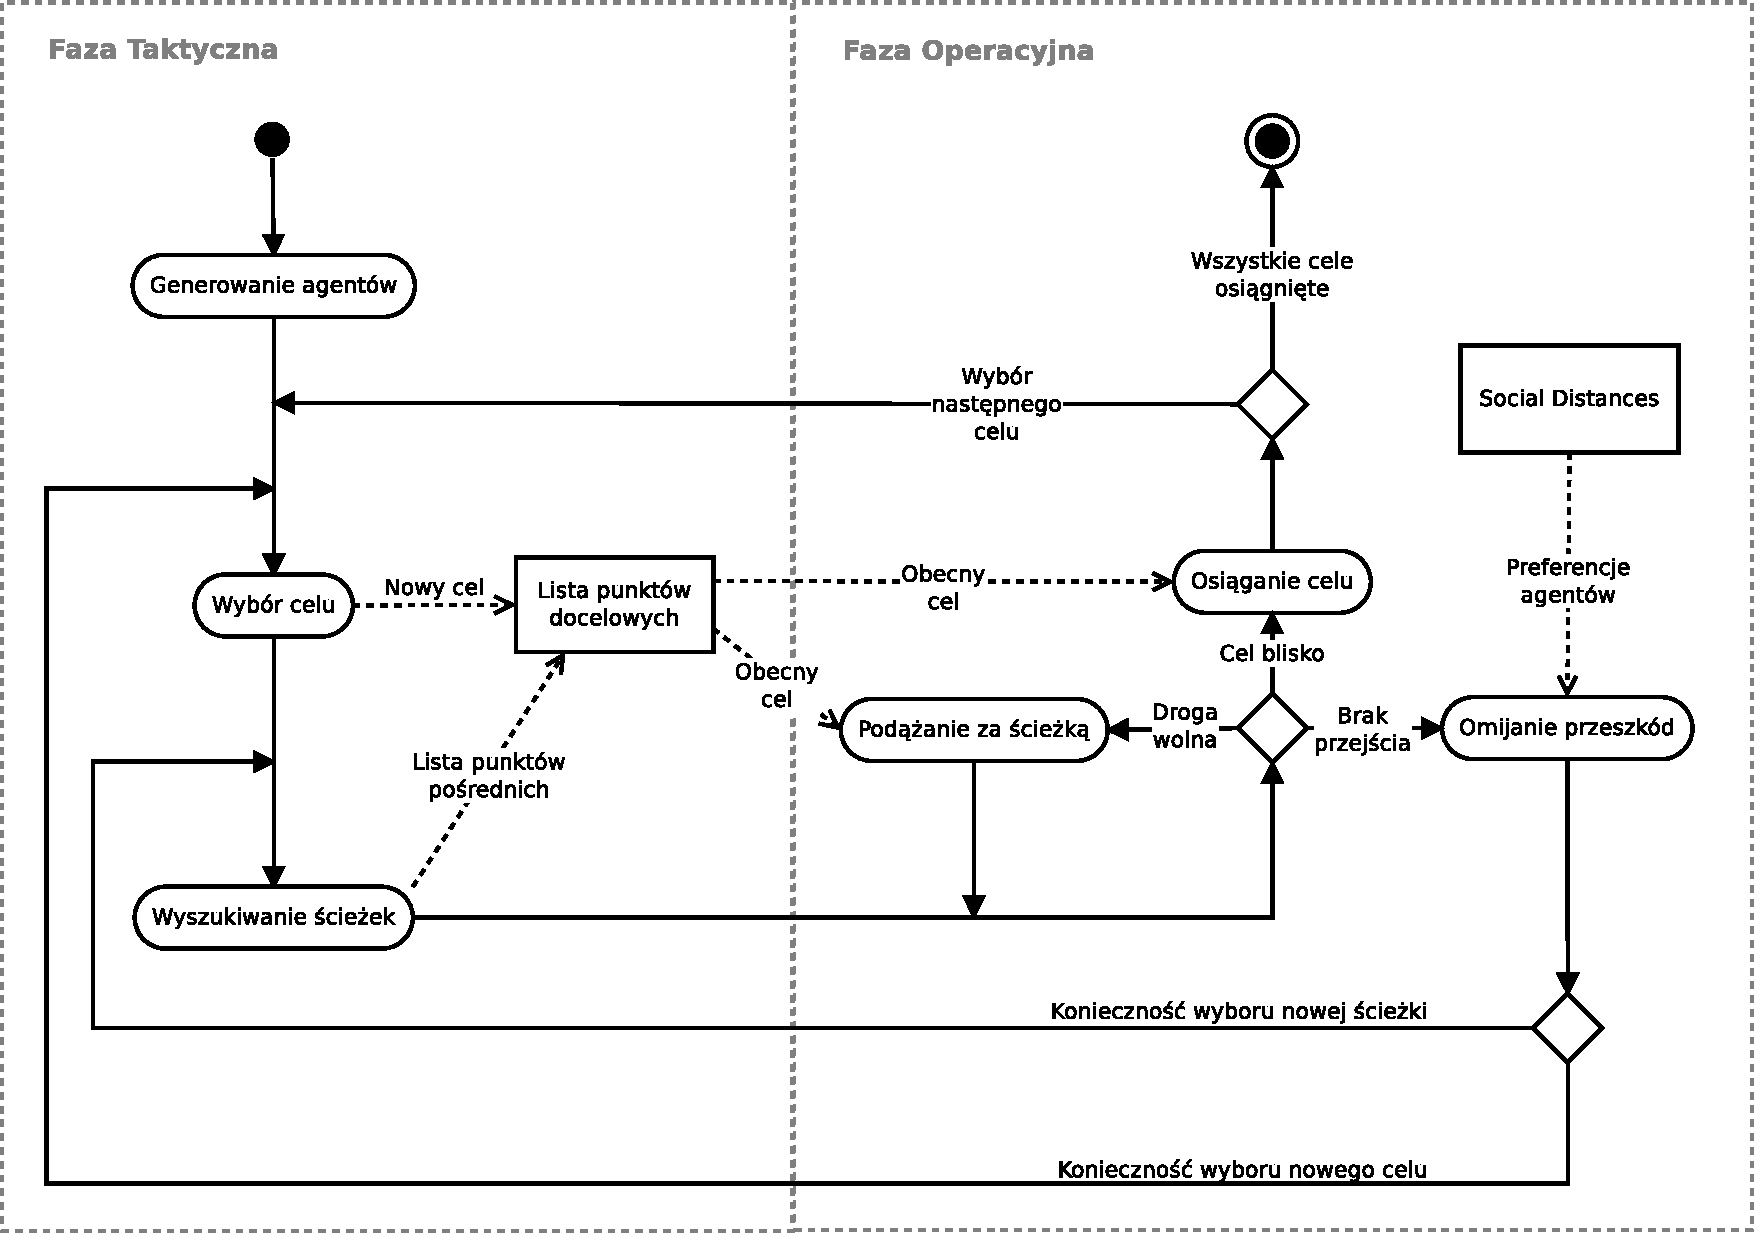
\includegraphics[scale=0.7]{./img/ActorActivity.pdf}
        \caption{Diagram aktywności agentów.}
        \label{fig:actor-activity}
    \end{figure}

Algorytm rozpoczyna pracę od wygenerowania agenta na podstawie wcześniej zdefiniowanych archetypów.
Dla każdego agenta wybierana jest wstępna lista miejsc docelowych, które zostaną przez niego odwiedzone w czasie działania symulacji, oraz obliczana jest optymalna ścieżka wiodące do pierwszego wybranego w poprzednim kroku miejsca docelowego. Algorytm następnie modyfikuje ścieżkę w oparciu o mapę rozkładu stref specjalnych centrum handlowego by lepiej modelować faktyczne zamiary danego aktora.

Po wygenerowaniu niezbędnych danych taktycznych dla każdego agenta algorytm przechodzi do fazy operacyjnej, która odpowiada za właściwe przemieszczanie agentów. Faza ta zachodzi w lokalnym otoczeniu każdego agenta i odpowiada za zachowania takie jak omijanie przeszkód, grupowanie się, podążanie za obraną ścieżką i inne akcje związane ze specjalnymi strefami centrum handlowego.
Algorytm na podstawie bezpośredniego otoczenia agenta oraz metadanych dotyczących obecnego celu jego podróży podejmuje decyzje o możliwości wykonania ruchu, lub w przypadku skrajnym o modyfikacji wybranej ścieżki prowadzącej do celu, czy nawet zmianie aktualnego celu podróży.
W przypadku osiągnięcia miejsca docelowego algorytm przechodzi do rozpatrywania następnego miejsca docelowego, lub w tryb ``błądzenia'', gdy osiągnięto już wszystkie wyznaczone cele.

\newpage
        \subsection{Faza taktyczna}
        \label{sec:tactical}

        \begin{figure}[H]
            \centering
            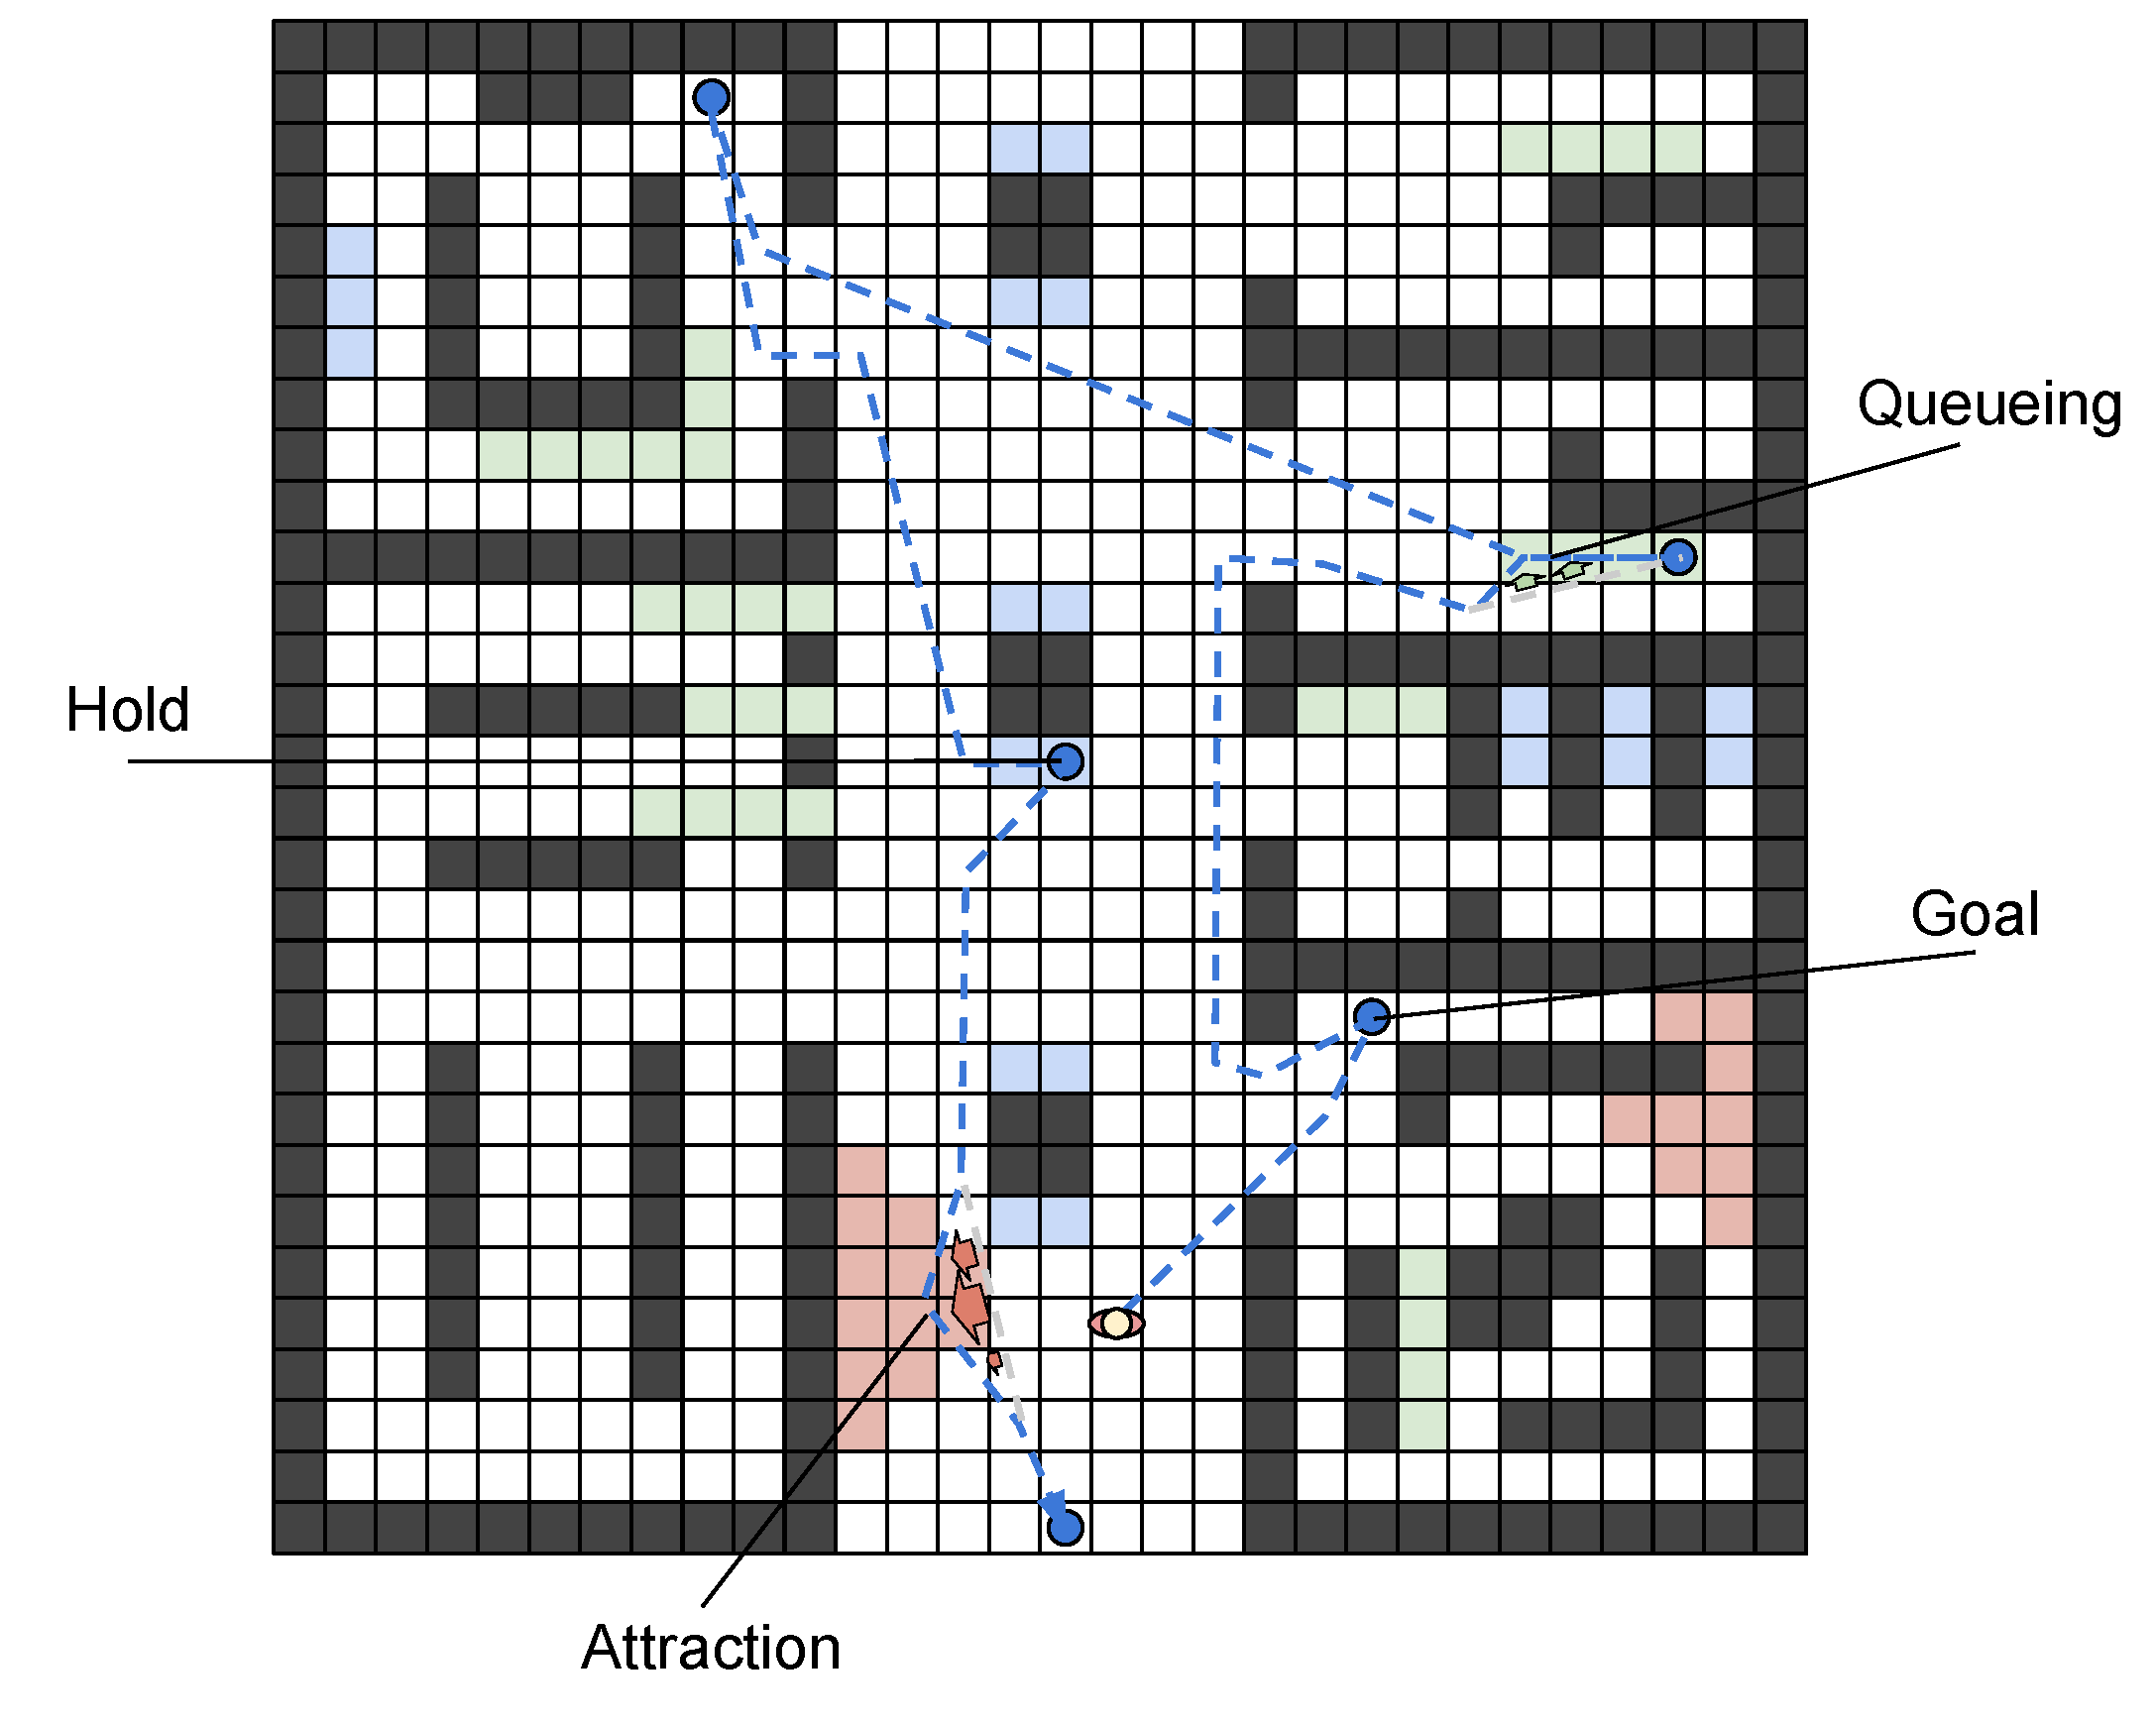
\includegraphics[scale=0.3]{./img/Tactical.pdf}
            \caption{Zakres operacji taktycznej części modelu ruchu.}
            \label{fig:tactical}
        \end{figure}

\noindent
Faza taktyczna zachodzi globalnie dla każdego agenta bez uwzględnienia jego lokalnego otoczenia, innych agentów, czy fizycznych właściwości centrum handlowego - nie jest istotnym, czy dany korytarz został zablokowany przez grupę ludzi i nie umożliwia przejścia. Faza ta modeluje abstrakcyjne zamiary agenta i jej celem jest przede wszystkim wybór listy miejsc docelowych oraz wyznaczenie dróg do nich prowadzących, co zostało osiągnięte dzięki \hyperref[sec:path-finding]{algorytmowi znajdowania ścieżek} oraz \hyperref[sec:mall-impl]{mapie rozkładu stref specjalnych} centrum handlowego. Cele podróży agentów wybierane są ze zbioru punktów szczególnego zainteresowania - punktów graniczących ze ścianami centrum handlowego. Przy wyznaczaniu ścieżek pod uwagę brane są \hyperref[sec:attractors]{atraktory}, \hyperref[sec:queues]{kolejki} i \hyperref[sec:entrance-exits]{przejścia}, które algorytm stara się osiągnąć modyfikując wcześniej wyznaczoną, optymalną ścieżkę prowadzącą do aktualnego celu podróży.

        \subsection{Faza operacyjna}
        \label{sec:operational}

        \begin{figure}[H]
            \centering
            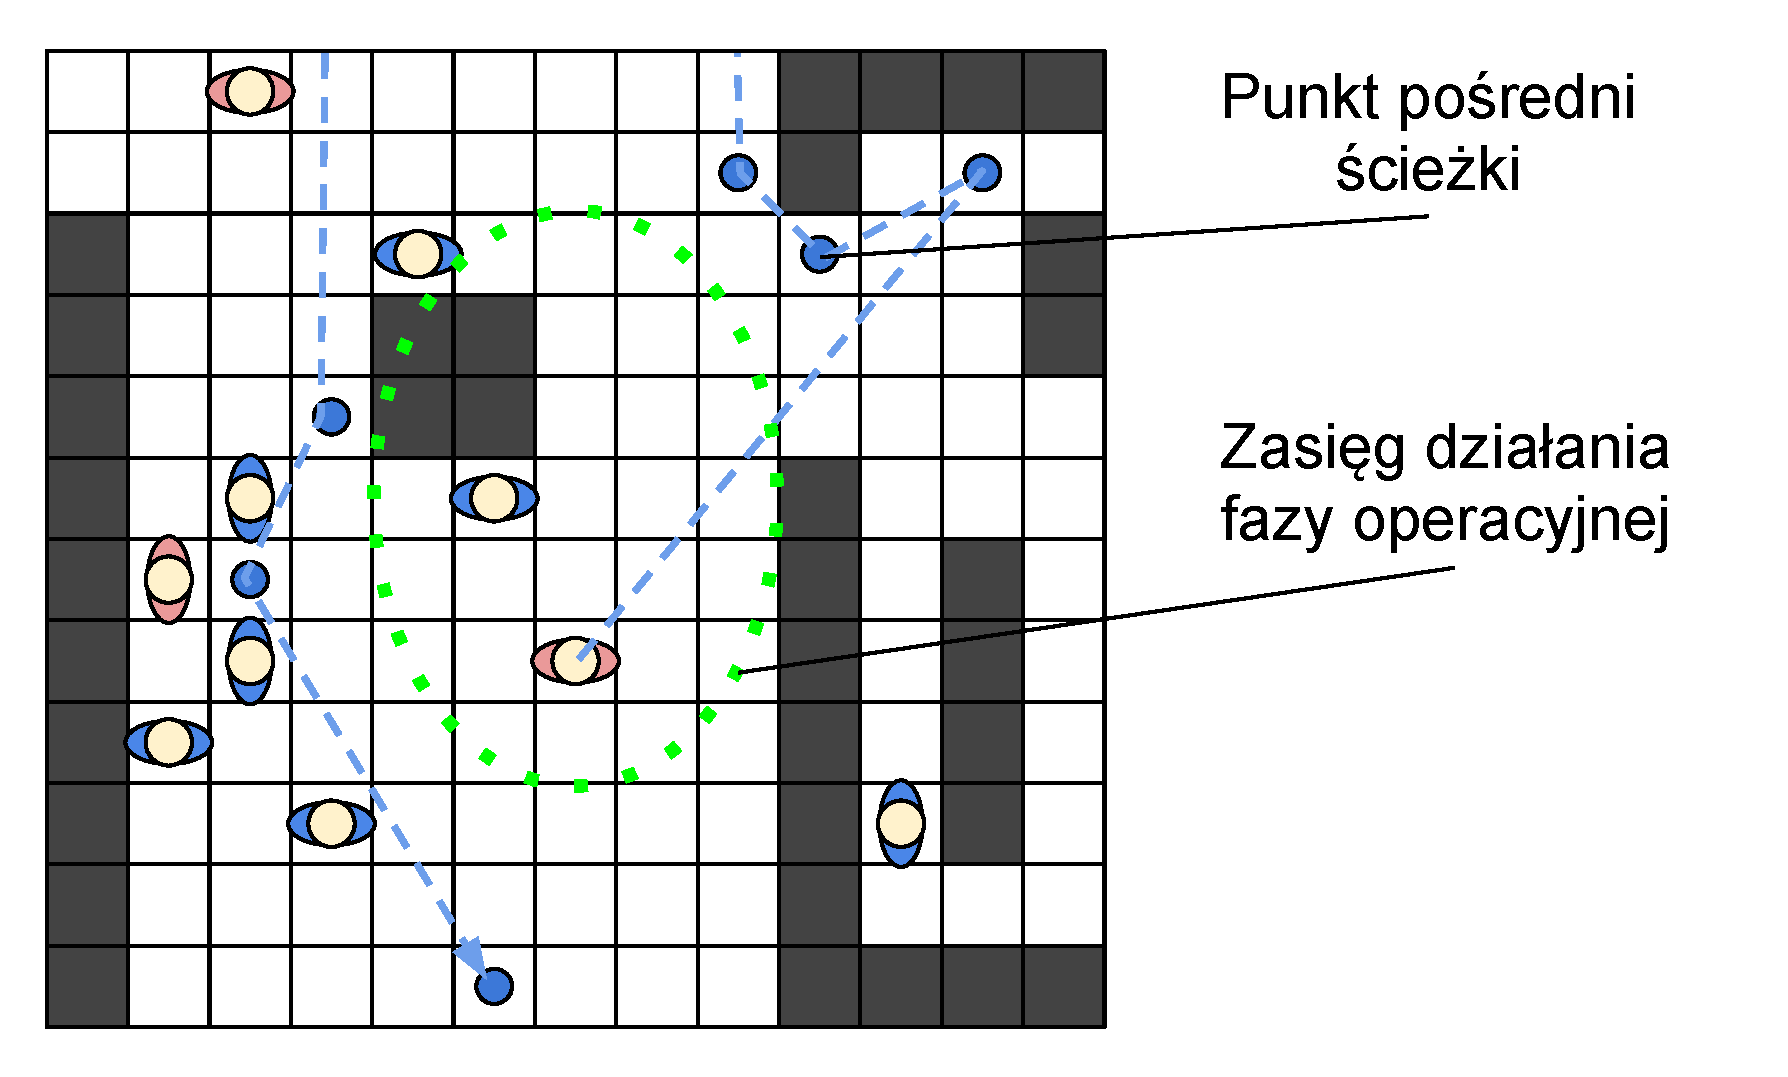
\includegraphics[scale=0.3]{./img/Operative.pdf}
            \caption{Zakres działania operacyjnej części modelu ruchu.}
            \label{fig:operational}
        \end{figure}

        % TODO Potrzeba większego opisu, który bardziej zagłębia się w wybrany algorytm operacyjny.

\noindent
Faza operacyjna zachodzi w lokalnym otoczeniu każdego agenta, a jej celem jest wykonanie właściwego ruchu agenta. Faza ta jest odpowiedzialna za unikanie kolizji i omijanie przeszkód. Pod uwagę brani są inni agenci oraz metadane dotyczące drogi prowadzącej do aktualnego celu podróży wygenerowane w taktyczniej fazie działania algorytmu. W implementacji fazy operacyjnej wykorzystano zmodyfikowane algorytmy \hyperref[sec:ped-4-impl]{Ped-4} i \hyperref[sec:social-force-impl]{Social-Force}. \\

\noindent
Oryginalny \textbf{Ped-4} został zaproponowany w pracy \textit{Modeling Four Directional Pedestrian Movements} (\cite{refs:4-way-movement}). Ponieważ prowadzi on do samoorganizowania się pieszych w kolumny, w symulacji galerii używany jest w odniesieniu do przestrzeni, po których ruch odbywa się w sposób uporządkowany (tj. do korytarzy, alejek oraz niewielkich skrzyżowań).

Algorytm składa się z następujących etapów:
\begin{enumerate}
\item dostosowanie kierunku ruchu \
	Gdy kąt między kierunkiem ruchu, a kierunkiem do celu przekroczy wartość graniczną, pieszy skręca w stronę celu.
\item zmiana pasa ruchu \
	Obliczana jest ilość wolnych pól dla obecnie zajmowanego pasa i dla pasów sąsiednich. Pieszy zajmuje ten pas, który na chwilę obecną umożliwia mu przesunięcie się o największą ilość pól do przodu. Przy wyborze preferowany jest dotychczasowy pas. W przypadku, gdy obecnie zajmowany pas nie jest ``czysty'' (tzn. z naprzeciwka idzie inny pieszy), aby uniknać kolizji pieszy stara się ``schować'' za inną osobą idącą w tym samym co on kierunku.
\item krok naprzód \
	W przypadku, gdy pole bezpośrednio przed pieszym (zgodnie z kierunkiem ruchu) jest wolne - próba zajęcia go. Jeśli nie jest to możliwe - próba dokonania zamiany miejsca z innym pieszym. Wymiana odzwierciedla sytuację, gdy piesi ``skręcają tułowie'', by ``przecisnąć się'' obok siebie. Etap \textit{krok naprzód} powtarzany jest wielokrotnie, dopóki nie skończą się ``punkty ruchu'' pieszego.
\end{enumerate}

Poniżej zamieszczono preferowaną kolejność dokonywania zamian:
\begin{enumerate}
\item między pieszymi idącymi w przeciwnych kierunkach na tym samym pasie
\item między pieszymi idącymi w przeciwnych kierunkach na sąsiednich pasach (na polach po przekątnej)
\item między pieszymi idącymi w kierunkach prostopadłych względem siebie (na polach po przekątnej)
\item między pieszymi idącymi w kierunkach prostopadłych względem siebie (jeden ``tarasuje'' drugiemu drogę)
\end{enumerate}

Pieszy może wybrać daną możliwość tylko wtedy, gdy jego ``partner'' do zamiany nie wykonał jeszcze swojego ruchu. Jeśli dana wymiana nie dojdzie do skutku, próbowana jest kolejna opcja z listy (znajduje to potwierdzenie w obserwacjach - w sytuacji dużego tłoku ludzie chętniej dokonują takich manewrów).

\noindent
Algorytm \textbf{Social Force} opiera się na obserwacji, że każdy człowiek posiada wokół siebie (głównie przed sobą) tzw. \textit{strefę komfortu}, w której niechętnie widzi osoby postronne. Po zsumowaniu stref komfortu wszystkich agentów otrzymuje się swoisty rozkład potencjału, na podstawie którego wyznaczany jest ich dalszy kierunek ruchu. Zasada, według której odbywa się ruch, jest prosta - dojść do celu po polach o jak najmniejszym potencjale. Jeśli w danym momencie brak jest dostępnych pól, pieszy ``drepcze'' w miejscu w oczekiwaniu na zwolnienie się któregoś z nich. Algorytm \textit{Social Force} służy głównie do modelowania miejsc, w których ludzie ``wałęsają się'', jak place czy wnętrza sklepów.

\newpage
    \section{Implementacja}
    \label{sec:implementation}

     % TODO Opisać technikalia implementacji...

        \subsection{Reprezentacja centrum handlowego}
        \label{sec:mall-impl}

        \begin{figure}[H]
            \centering
            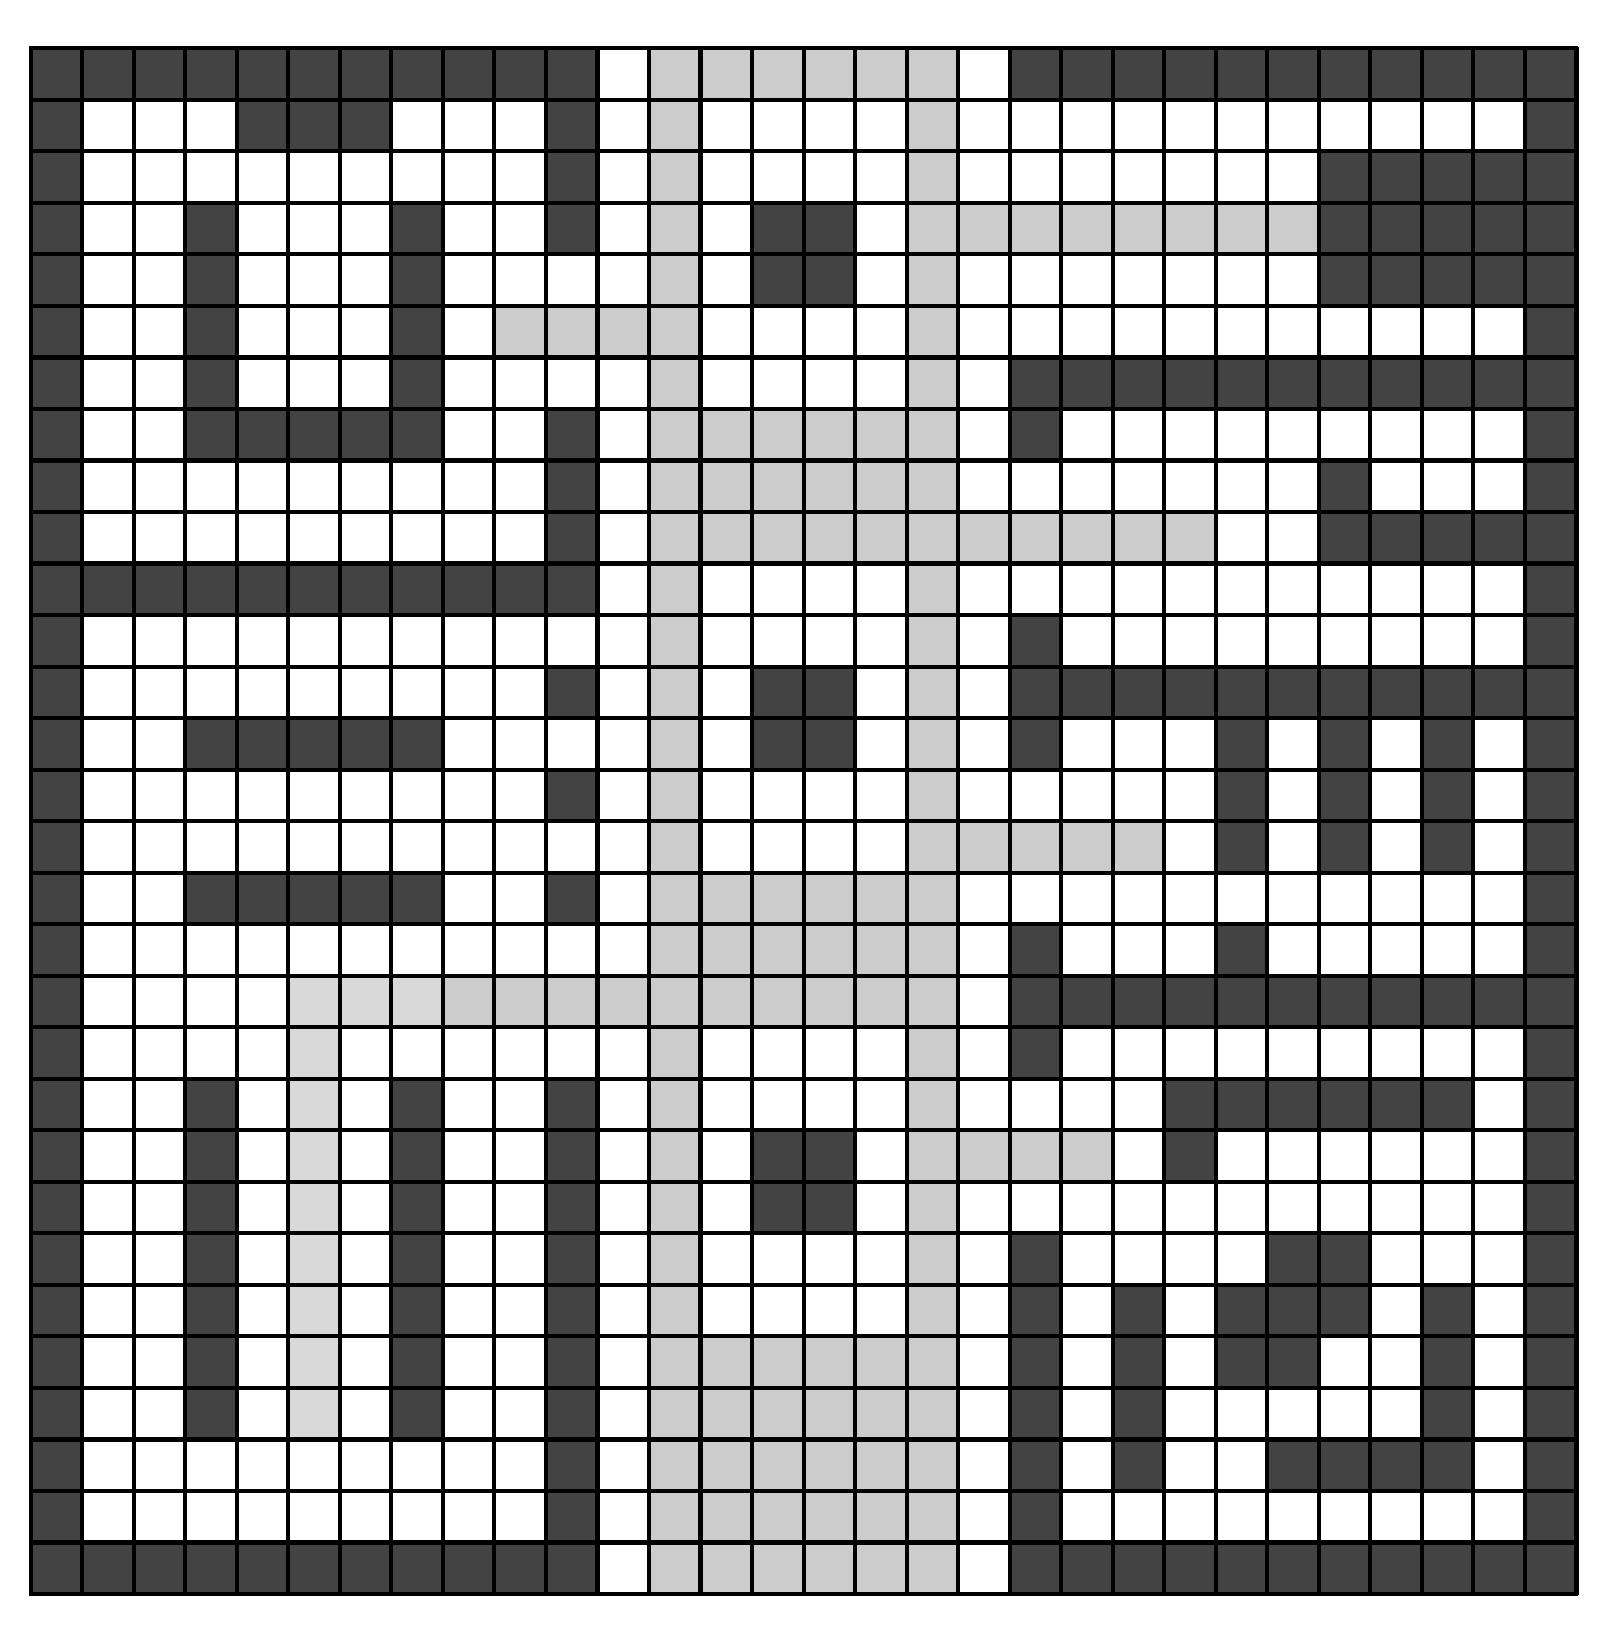
\includegraphics[scale=0.2]{./img/MallLayout.pdf}
            \caption{Przykładowy rozkład pomieszczeń małego centrum handlowego.}
            \label{fig:mall-layout}
        \end{figure}

        \begin{figure}[H]
            \centering
            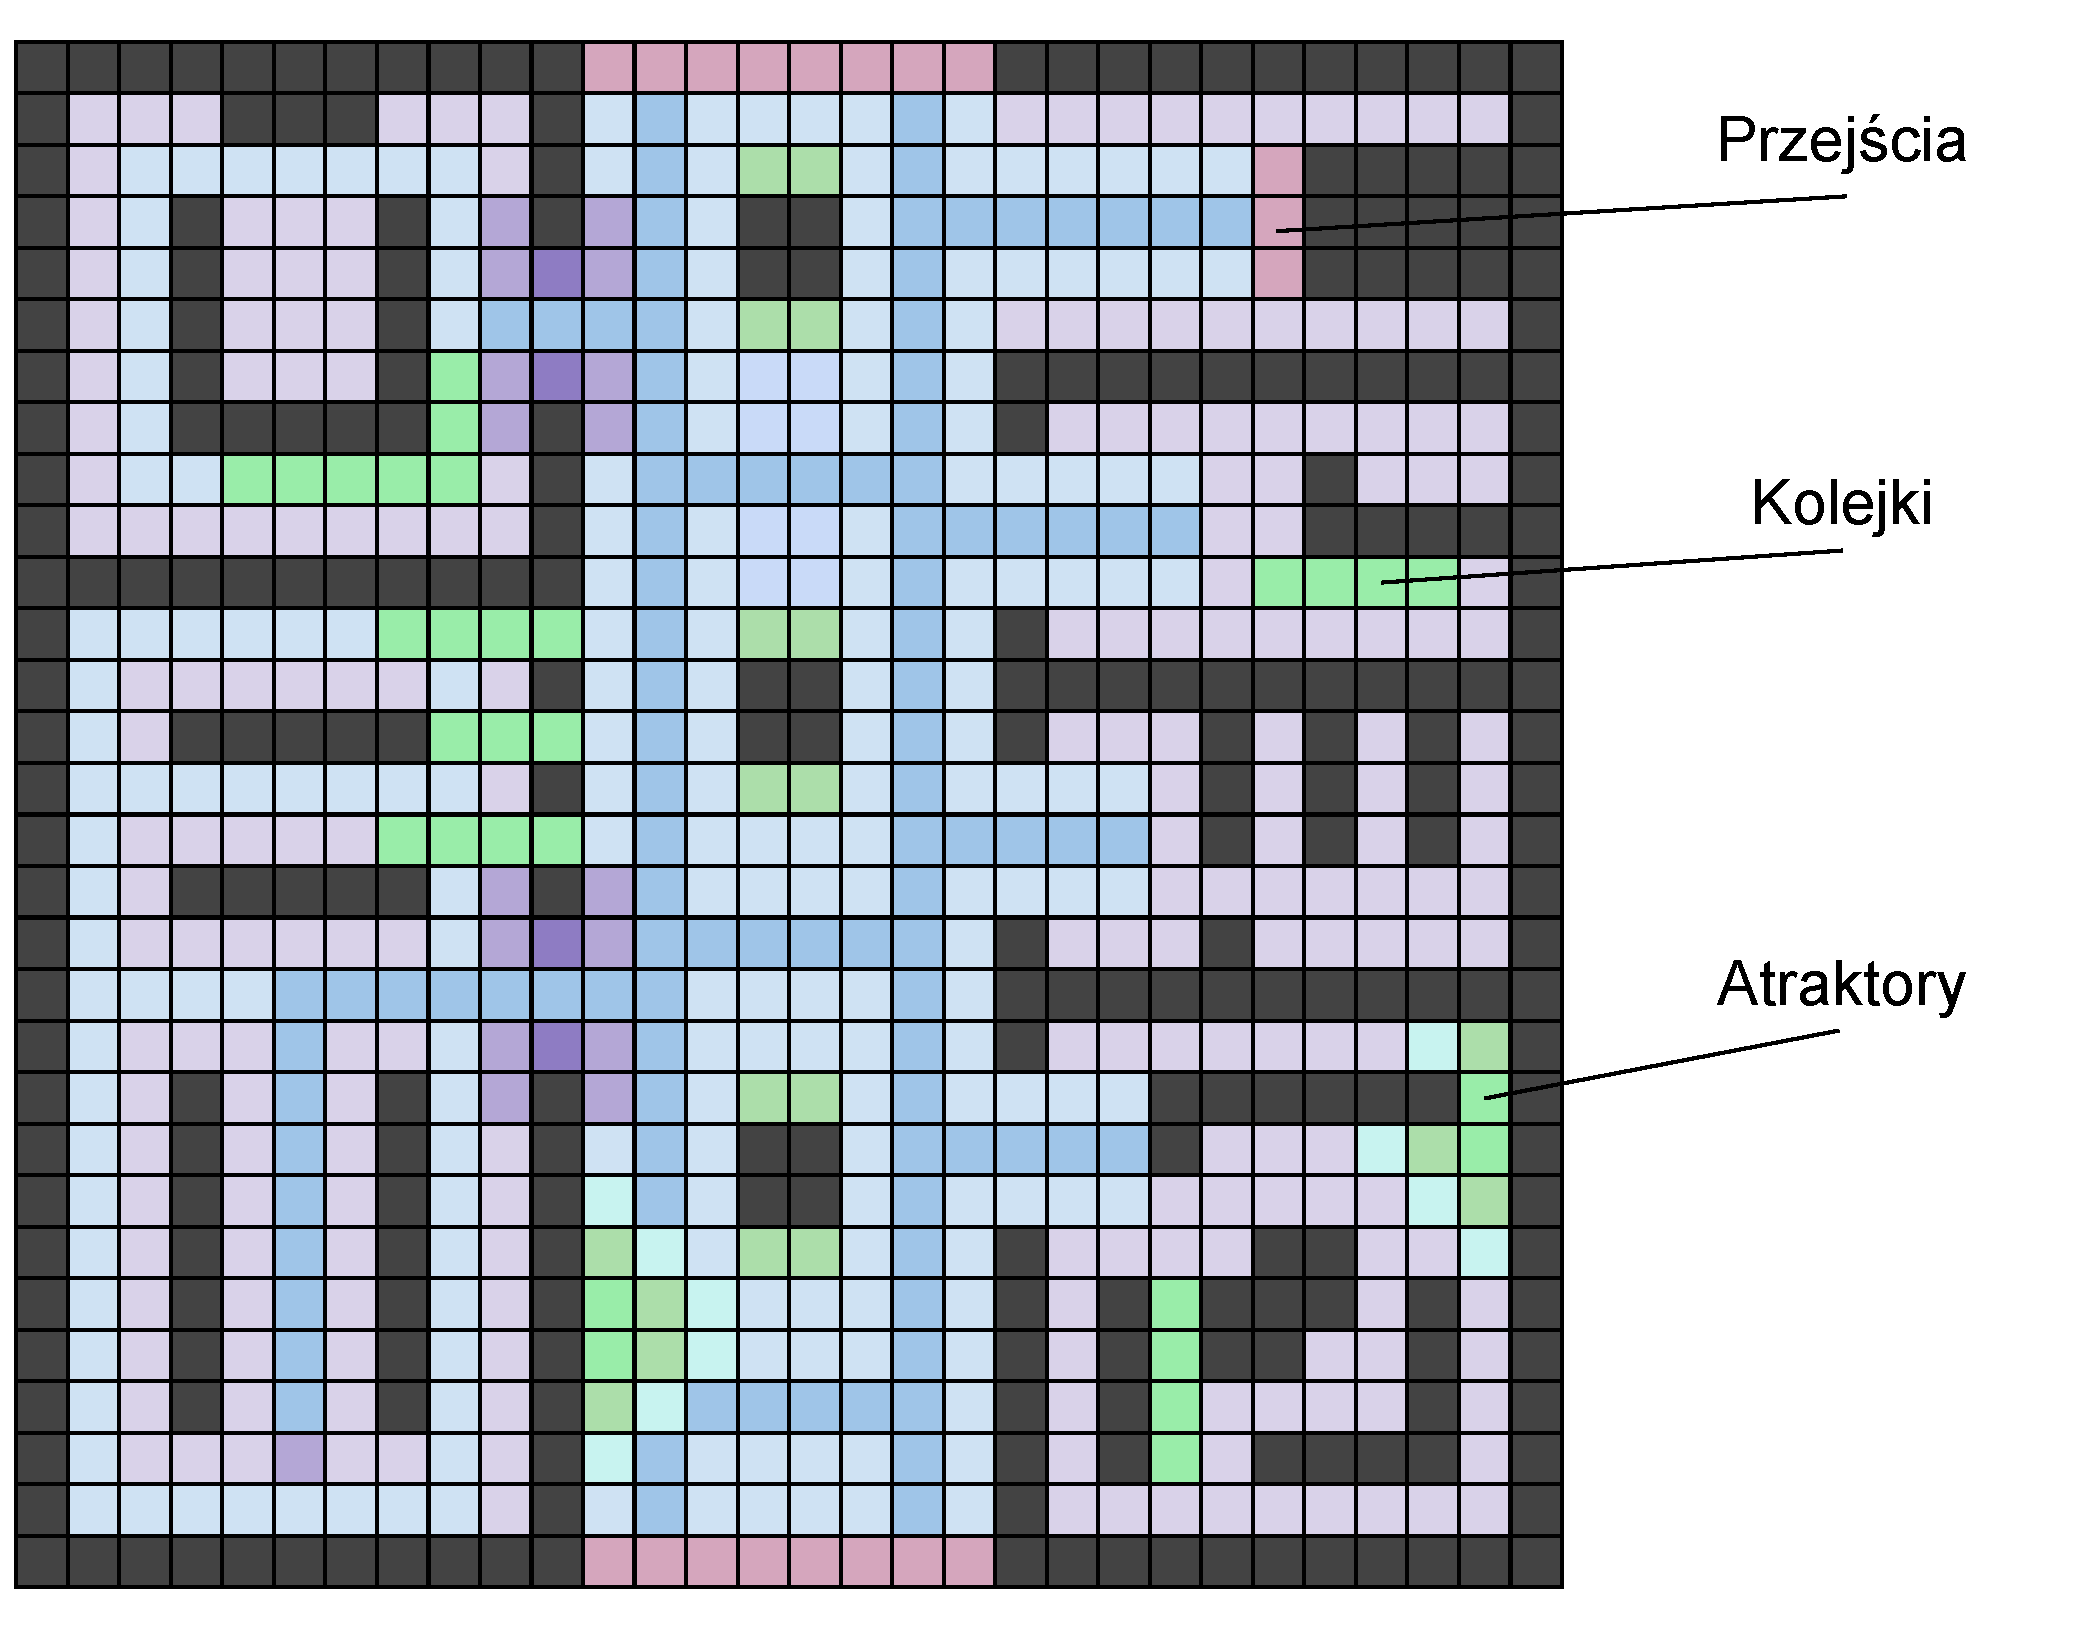
\includegraphics[scale=0.2]{./img/MallFeatures.pdf}
            \caption{Przykładowy rozkład stref specjalnych małego centrum handlowego.}
            \label{fig:mall-features}
        \end{figure}

        % TODO Opisać jak obsługiwane są wielopiętrowe centra handlowe.
        % TODO Opisać, jak kodowane są poszczególne strefy specjale.

        \subsection{Reprezentacja agentów}
        \label{sec:actor-impl}

        % TODO Opisać parametry agentów.

        \subsection{Wybór puntków docelowych}
        \label{sec:destination-choice}

        % TODO Opisać, jak wybierane są punkty docelowe.

        \subsection{Znajdowanie ścieżek}
        \label{sec:path-finding}

        % TODO Opisać algorytm A*.

        \subsection{Dewiacja ścieżek}
        \label{sec:path-deviation}

        % TODO Opisać wpływ różnych stref specjalnych na wygenerowane ścieżki.

        \subsection{Ruch agentów}
        \label{sec:movement-impl}

        \subsection{Ped-4}
        \label{sec:ped-4-impl}

        \subsection{Social Force}
        \label{sec:social-force-impl}

\newpage
    \section{Symulacja i analiza wyników}
    \label{sec:sim}

    % TODO Stworzyć i opisać przykładowy problem (albo dwa), takie jak mały sklep, czy duże centrum.
    % TODO Zasymulawać przykładowy problem i zebrać dane.

        \subsection{Kalibracja i walidacja parametrów symulacji}
        \label{sec:p}

        % TODO Opisać metody kalibracji i walidacji parametrów symulacji.

        \subsection{Uzyskane wyniki ilościowe i jakościowe}
        \label{sec:results}

        % TODO Opisać otrzymane wyniki, przedstawić statystyki zachowań,
        % TODO czasów spędzonych w centrum handlowym itp.

        \subsection{Wyniki symulacji a rzeczywistość}
        \label{sec:sim-vs-reality}

        % TODO Napisać dokładne porównanie z rzeczywistymi danymi.

\newpage
    \begin{thebibliography}{9}
        \label{sec:refs}

        \bibitem[Wąs, Gudowski, Matuszyk 2006]{refs:social-distances-1} - Social Distances Model of Pedestrian Dynamics
        \bibitem[Karakayali 2009]{refs:social-distances-2} - Social Distance and affective orientation
        \bibitem[Blue, Adler 2000]{refs:4-way-movement} - Modelling Four Directional Pedestriam Movements
        \bibitem[Blue, Adler 2001]{refs:cellular-movement} - Cellular automata microsimulation for modeling bi-directional pedestrian walkways
        \bibitem[Bitgood, Dukes 2005]{refs:movement-economy} - Economy of Movement and Pedestrian Choice Point Behavior in Shopping Malls
        \bibitem[Borgers, Timmermans 1986]{refs:route-choice-1} - A Model of Pedestrian Route Choice and Demand for Retail Facilities within Inner-City Shopping Areas
        \bibitem[Borgers, Timmermans 1986]{refs:route-choice-2} - City centre entry points, store location, patterns and pedestrian route choice behaviour: a microlevel simulation model
        \bibitem[Borgers, Timmermans 2005]{refs:pedestrian-behaviour-1} - Modelling pedestrian behaviour in downtown shopping areas
        \bibitem[Kitazawa, Batty 2004]{refs:pedestrian-behaviour-2} - Pedestrian Behaviour Modelling - An Application to Retail Movements using a Genetic Algorithm
        \bibitem[Zacharias 2000]{refs:real-data-1} - Shopping behavior at Alexis-Nihon Plaza in Montreal
        \bibitem[Rauh, Schenk, Schrődl 2011]{refs:real-data-2} - The Simulated consumer - an agent-based approach to shopping behaviour
        \bibitem[Helbing 1992]{refs:fluid-dynamics} - A Fluid Dynamic Model for the Movement of Pedestrians
    \end{thebibliography}
\end{document}
